\documentclass[10pt,conference,compsocconf]{IEEEtran}
\usepackage{booktabs}
\usepackage{hyperref}
\usepackage{graphicx}	% For figure environment
\usepackage{subcaption}
\usepackage{amsmath}
\usepackage{bm}
\usepackage{tikz}
\usepackage{tikz-qtree}
\usepackage{amsmath}
\usepackage{amssymb}
\usepackage{amsfonts}
\usepackage{amsthm}
\usepackage{mathrsfs}
\usepackage{cleveref}
\usepackage{xcolor}
\usepackage{nicefrac}
\usetikzlibrary{trees,calc,arrows.meta,positioning,decorations.pathreplacing,bending}


\begin{document}
\title{Deep Learning - Miniproject 2}

\author{
  Olesia Altunina (285467), Mauro Pfister (235440), Joey Zenhaeusern (226652)
}

\maketitle

\begin{abstract}
This report is a description of our approach to implement a simple deep-learning framework from scratch and particularly without using PyTorch's automatic differentiation. The framework contains all the necessary tools to create, train and evaluate a simple network. The functionality is demonstrated by building a classification network for a randomly generated dataset. 
\end{abstract}

\section{Introduction}

\section{Framework implementation}
In order to implement our own mini deep-learning framework MyTorch we chose a structure based on the suggestion provided in the project description. All modules are implemented as classes which inherit from a parent class \texttt{Module}. They need to override the \texttt{forward()}, \texttt{backward()} and \texttt{param()} methods.

MyTorch supports batch processing which significantly decreases training times as well as prediction times on large networks. Currently, we do not support multiple forward passes since the inputs are not saved into a buffer. While it is still possible to run several forward passes one should keep in mind that the backward pass will only calculate the gradients with respect to the last applied input.

\subsection{Linear module}
The linear module implements a simple fully connected layer with or without bias. Following the suggestion of Glorot and Bengio \cite{pmlr-v9-glorot10a}, weights and biases are initialized with a normal distribution of zero mean and standard deviation $\sigma$ given by
\begin{equation} \label{eq:Winit}
  \sigma = \sqrt{2 / (n_{in} + n_{out})},
\end{equation}
where $n_{in}, n_{out}$ denote the input and output features respectively.\\

If the back propagation is carried out on a batch of samples, the gradients of the weights and the biases are averaged over the whole batch. This is in accordance with the official PyTorch implementation and ensures that the gradient norms do not grow with the batch size.

\subsection{Sequential module}
The sequential module takes a chronological list of other modules as input and groups them in one module for convenience. The forward pass sequentially executes the forward passes of the individual modules. The backward pass does the same but in reversed order.

\subsection{ReLU and Tanh module}
% TODO: what else can we write here?
Both ReLU and Tanh modules have no parameters.

\subsection{MSE loss module}
The \texttt{LossMSE} class implements a mean squared error loss function defined as follows:
\begin{equation} \label{eq:MSE}
  l(x,t) = \frac{1}{n} \sum_1^n{(x_i - t_i)^2}, 
\end{equation}
where $n$ defines the dimension of $x$ and $t$. Note that we currently do not support the computation of the loss over a batch.

\subsection{Optimizer}
Additionally to the required modules above we also defined an optimizer class \texttt{Optimizer} that can be used to implement different optimizers. It takes the parameters of a model as input and contains a \texttt{step()} method to perform a gradient step on the model parameters. A second method \texttt{zero\_grad()} can be used to set the gradients of all optimized parameters to zero. 

Currently, only a stochastic gradient descent optimizer \texttt{SGD} is available,that can be used with or without momentum. The implementation of momentum is based on the one in PyTorch which differs from Sutskever et. al. \cite{sutskever2013importance}. The update of parameter $p$ is defined as follows 
\begin{equation} \label{eq:SGDmoment}
  \begin{aligned}
    v &= \rho v + g \\
    p &= p - \alpha v,
  \end{aligned}
\end{equation}
where $\alpha$, $\rho$ and $g$ denote learning rate, momentum and parameter gradient respectively.

\section{Framework validation}
To ensure the correctness of our implementations we wrote a series of unit tests which compare the functionalities of our code to the corresponding PyTorch functionalities. Currently the forward and backward passes of \texttt{Linear}, \texttt{ReLU} and \texttt{Tanh} modules can be tested.

Additionally, we created the same network architecture once MyTorch and once in PyTorch and initialized all model parameters to a value of $10^{-6}$. This ensures that both models have exact the same initial condition. Using this initialization the total training loss per epochs does not differ by more than $10^{-6}$ and the training and test accuracies match perfectly. Therefore we conclude that within the limitations of our framework, the functionality is equivalent to PyTorch.

\section{Data description}
According to the task description the training and test data sets consist each of 1000 points sampled uniformly in $[0,1]^2$. Class 0 is defined by all the points outside the disk with radius $\nicefrac{1}{\sqrt{2\pi}}$ and center $(\nicefrac{1}{2}, \nicefrac{1}{2})$ while class 1 denotes all the points inside that disk (see Figure~\ref{fig:data_set}).

\begin{figure}[h]
  \centering
  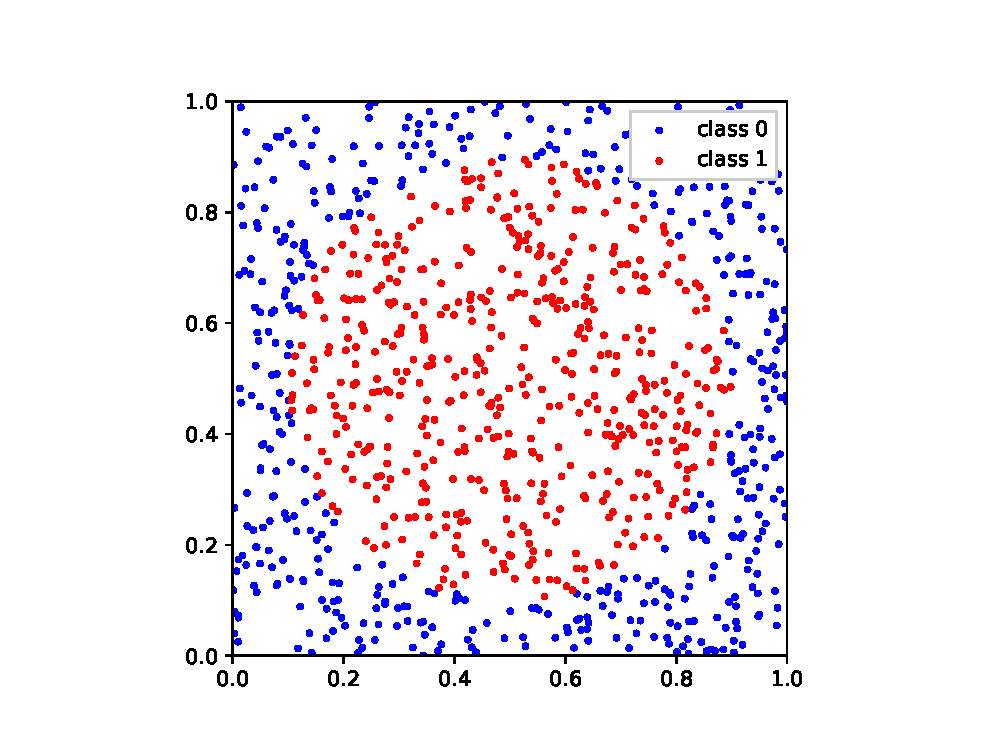
\includegraphics[width = 0.4\textwidth]{fig/disk_data_set.eps}
  \caption{Visualization of data set.}
  \label{fig:data_set}
\end{figure}


\section{Network description}
The network used for classification of the data set consists of two input units, three hidden layers of 25 units and two output units. We chose to use ReLU as activation functions for all layers.

\section{Performance evaluation}
% TODO: mention that for 25 epochs there is quite a bit of variation for both models -> might be due to weight initialization
When training the model we noted that the error and loss values would vary by quite a lot. Figure~\ref{fig:err} and Figure~\ref{fig:err2} depict the test and train error comparison of the same model trained in MyTorch and Pytorch over 25 epochs. We suspect that this variation is due to the random nature of the data (which is newly generated on every run) and the randomness in the weight initialization. Overall our framework performs very similar to the python reference implementation.
\begin{figure}[h]
  \centering
  \includegraphics[width=0.4\textwidth]{fig/err.pdf}
  \caption{Test and train error over 25 epochs.}
  \label{fig:err}
\end{figure}

\begin{figure}[h]
  \centering
  \includegraphics[width=0.4\textwidth]{fig/err2.pdf}
  \caption{MyTorch vs. PyTorch loss over 25 epochs.}
  \label{fig:err2}
\end{figure}

In Table~1 we can see the test error results after running the model 10 times. Surprisingly our model manages to achieve a slightly lower test error in the mean as well as slightly lower standard deviation.
\begin{table}[]
    \centering
\begin{tabular}{@{}lllll@{}}
\toprule
        & Test error (mean) & Test error (std) \\ \midrule
MyTorch & 4.0               & 6.5 \%           \\
PyTorch & 5.3               & 7.9 \%          
\end{tabular}
  \caption{Test error results after running model 10 times}
\end{table}
% TODO: plot the prediction of the model on the data set -> maybe run 10 times and even show std ?


\bibliographystyle{IEEEtran}
\bibliography{literature}

% reference to Bishop for Newton's method

\end{document}
